\documentclass[10pt,conference,compsocconf]{IEEEtran}

\usepackage{hyperref}
\usepackage{graphicx}	% For figure environment

% Packages added by Joachim

%drow graph
\usepackage{fancybox}
\usepackage{tikz}
\usepackage{capt-of}
\usepackage{verbatim}

% cancel math expression
\usepackage{cancel}

% math
\usepackage{amsmath}

% url
\usepackage{hyperref}

%subfigure
\usepackage{subcaption}
\usepackage{cleveref}

% multiline tabular cell
\newcommand{\specialcell}[2][c]{%
  \begin{tabular}[#1]{@{}l@{}}#2\end{tabular}}



\begin{document}
\title{PCML CS-433: Recommender System}

\author{
  Gael Lederrey, SCIPER 204874, gael.lederrey@epfl.ch \\
  Stefano Savar\`e, SCIPER 260960, stefano.savare@epfl.ch \\
  Joachim Muth, SCIPER 214757, joachim.muth@epfl.ch\\ \\
  \textit{School of Computer and Communication Sciences, EPF Lausanne, Switzerland}
}

\maketitle

%========================
\begin{abstract}

\end{abstract}

%========================
\section{Data description}

The data represent ratings from $10'000$ users on $1'000$ movies in an integer scale from 1 to 5. This scale represent the number of \textit{stars} given by the users, 1 being the lowest grade and 5 the best.

The training set used to train our algorithm contains $1'176'952$ ratings which represent around 12\% of possible filled ratings. 
An other $1'176'952$ ratings are hidden from us and must be predicted by our recommender algorithm.


%\begin{figure}[htbp]%------- PICTURE---------
%  \centering
%  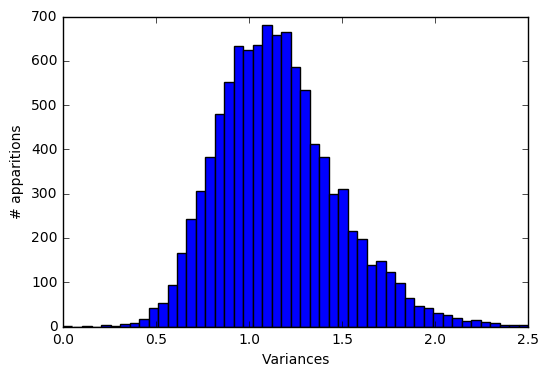
\includegraphics[width=0.9 \columnwidth]{img/Variances}
%  \caption{Distribution of variances of ratings per user.}
%  \vspace{-3mm}
%  \label{fig:denoise-fourier}
%\end{figure}
%\begin{figure}[htbp]
%  \centering
%  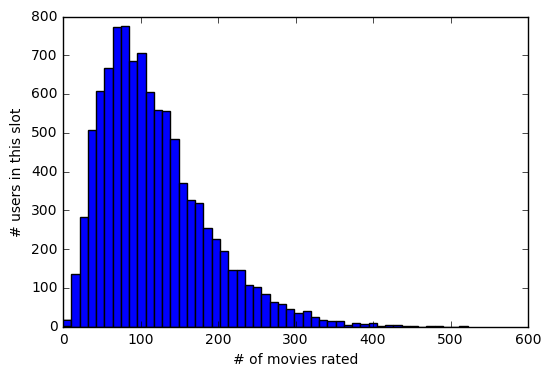
\includegraphics[width=0.9 \columnwidth]{img/Ratings}
%  \vspace{-3mm}
%  \caption{Number of movies rated per user.}
%  \label{fig:denoise-wavelet}
%\end{figure}


\begin{figure}[tbp] %-------------- FIGURE -------------
    \centering
    \hspace{-0.6cm}
    \begin{subfigure}[t]{0.45\columnwidth}
        \centering
        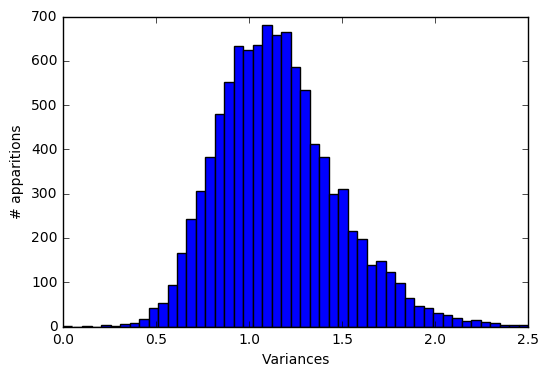
\includegraphics[height=1.2in]{img/Variances}
        \vspace{-3mm}
  \caption{Distribution of variances of ratings per user. No spammers.}
  \label{variances}
    \end{subfigure}%
    \hspace{0.4cm}
    \begin{subfigure}[t]{0.45\columnwidth}
        \centering
        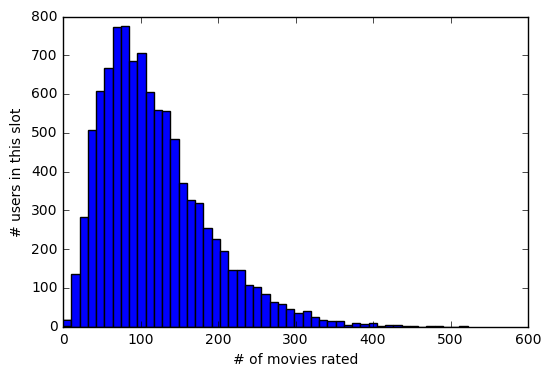
\includegraphics[height=1.2in]{img/Ratings}
        \vspace{-3mm}
        \caption{Number of movies rated per user. Good user participation.}
        \label{number_ratings}
    \end{subfigure}
    \caption{Statistical description of data}
\end{figure}


%========================
\section{Data exploration}

\subsection{Search for spammers}

One of the first step before starting learning from data is to ensure that they are real ones, and not produced by bots (spammers). As we know spammers can act in different ways: \textbf{uniform spammer} constantly rates movie in the same way, while \textbf{random spammers} randomly rates movies. In order to check their existence, we analyzed the variances of user ratings: uniform spammer would be put in evidence by null variance, while random spammer will present abnormally high variance. Figure (\ref{variances}) shows the gaussian distribution of the rating variances and ensure the data are free of spammers.

\subsection{Participation of users}

Even free of spammers, data can still contains \textbf{inactive users}, i.e. users which subscribed to a plateform but never use it or never rate movies. If they are in too big number compared with active user, they can disturb learning algorithms. Figure (\ref{number_ratings}) shows histogram of number of movies rated by users and confirm us the good participation of the users.

\subsection{User "moods"}

Because of mood/education//habits users having the same appreciation of a movie can rate it differently. Indeed, we show in figure (\ref{mood}) that some users systematically rate lower/higher that others. It's important to take this effect into account in both evaluation of a movie and recommendation for the user and proceed to a normalization of the ratings.



\begin{figure}[htbp] %-------------- FIGURE -------------
  \centering
  \includegraphics[width=\columnwidth]{img/deviation_mean}
  \caption{Difference of mean rating per user compared with overall mean.}
  \vspace{-3mm}
  \label{mood}
\end{figure}

%========================
\section{Model selection}

\subsection{Models description}
\subsubsection{Global mean/median}

The most simple model is to take all the ratings in the train set and apply the mean or the median value. We return this value as the prediction. This give a baseline from which we can compare further model.

\subsubsection{User/Movie mean/median}

Another simple model is to compute the mean or median value for the users or the movies.

\subsubsection{Movie mean/median with User mood}

The third set of model uses the mean or median value for each movie. We also compute the ``mood'' of the users this way:

\begin{equation}
 d_u = \overline{U} - \overline{u} \quad \forall u\in U
\end{equation}
where $\overline{U} = \frac{1}{\#U} \sum_{u\in U} \overline{u}$ and $\overline{u}$ being the average rating of the user $u$.

Then, we return the prediction of a user $u$ on a movie $m$:
\begin{equation}
 p_{m,u} = \overline{m} + d_u
\end{equation}
where $\overline{m}$ is either the mean or the median of the ratings on the movie $m$.

\subsubsection{Matrix Factorization using Stochastic Gradient Descent}
\subsubsection{Alternativ Least Square}
\subsubsection{kNN item-based}
\subsubsection{Pareto Dominance and Collaborative Filtering Nearest Neighbors}

\subsection{Models benchmark}

\begin{table}[htbp]
\centering
\begin{tabular}[c]{| l r |}
\hline
Model & RMSE \\
\hline 
\hline
Global mean					& 1.11906	\\
Global median 					& 1.12812	\\
User mean 					& 1.09520 \\
User median					& 1.15163 \\
Movie mean					& 1.03045 \\
Movie mean (mood norm.)		& 0.99653 \\
Movie median					& 1.09963 \\
Movie median (mood norm.)		& 1.05793 \\
MF-SGD 						& 1.00052 \\
MF-SGD (mood normalization) 		& 0.99981 \\
ALS							& 0.98861 \\
Collab. Filtering					& 1.02733 \\
\hline


\end{tabular}
  \caption{Benchmark of models.}
  \label{benchmark}
\end{table}




\subsection{Blending}

The \textit{Bellkor's Pragmatic Chaos} team, winner of 2009 \textit{Netflix Prize} explain in its paper that its solution was obtained by blending a hundred of different models. \cite{BellKore_netflix} Without having the same amout of models, we proceed the same to obtain our final solution. We performe a weighted sum that we optimize using \textbf{Nelder-Mead} method provided by \texttt{scipy.optimize} library. Initial weights are $1$ for each method and the final weights are listed in table (\ref{blending})





\begin{table}[htbp]
\centering
\begin{tabular}[c]{| l l l |}
\hline
Model & weight & parameters\\
\hline 
\hline
Global mean					& -0.64503			& -	\\
Global median 					& 4.16579				& -	\\
User mean 					& -3.67733			& - \\
User median					& -0.00498			& - \\
Movie mean					& 0.58294				& - \\
Movie mean (mood norm.)		& -0.43266			& - \\
Movie median					& -4.29733			& - \\
Movie median (mood norm.)		& 4.29873				& - \\
MF-SGD 						& -0.03862			& \specialcell[t]{$\gamma = 0.004$ \\
													 features = 20 \\
													 iterations = 20 \\
													 initial matrix = global\_mean} \\
MF-SGD (mood normalization) 		& -0.06728			& \specialcell[t]{$\gamma = 0.004$ \\
													 features = 20 \\
													 iterations = 20\\
													 initital matrix = global\_mean} \\
ALS							& 0.89273				& \specialcell[t]{$\lambda = 0.081$ \\
													 rank = 8 \\
													 iterations = 24} \\

Collab. Filtering					& 0.07109				& \specialcell[t]{$\alpha = 19$ \\
													 features = 20} \\
\hline

\end{tabular}
  \caption{Blending of models.}
  \label{blending}
\end{table}


%========================
% \section{Discussion}



%========================
\section{Result}

\section{Discussion}


\bibliographystyle{IEEEtran}
\bibliography{literature}

\end{document}
